\documentclass[twocolumn]{article}
\usepackage[utf8]{inputenc}
\usepackage[russian]{babel}
\usepackage{amsmath}
\usepackage{amsfonts}
\usepackage{amssymb}
\usepackage{graphicx}
\usepackage{lipsum}
\usepackage{multicol}
\usepackage{caption}
\usepackage{float}
\renewcommand{\thefootnote}{\fnsymbol{footnote}}
\renewcommand{\footnoterule}{
  \kern -3pt
  \hrule width \columnwidth height 0.5pt
  \kern 2.6pt
}
\usepackage{multicol} % Многоколоночный текст
\usepackage{fancyhdr}
\usepackage{rotating} % Для использования rotatebox

% Настройка стиля страницы
\pagestyle{fancy}
\fancyhf{} % очистить все заголовки и колонтитулы
\renewcommand{\headrulewidth}{0pt} % убрать линию в заголовке
\fancyfoot[R]{\bfseries\thepage} % жирная нумерация страниц в правом нижнем углу

\begin{document}

\twocolumn[
{\begin{minipage}{\textwidth}
%\vspace*{-2cm}
\rule{\textwidth}{0.4pt}
\begin{minipage}[b]{0.5\textwidth}
\centering

\includegraphics[width=0.4\textwidth]{logo.png} % Выравнивание логотипа по центру первой колонки
\end{minipage}%
\hfill
\begin{minipage}[b]{0.5\textwidth}
\begin{flushright}
\textbf{\Large Вычисление многочленов —\\[12pt] от Ньютона до наших дней}\\
\end{flushright}
\hspace{1cm}\textit{Э. Г. Белага}\\
\end{minipage}
\rule{\textwidth}{0.4pt}
\vspace{2ex}
\end{minipage}}
]


\section*{§ 1. Многочлены -- инструмент вычислителя}
\begin{quote}
\small\textit{Ну, начнем! Когда мы доберемся до 
этой истории, оноем знать
больше, чем теперь.}

\hfill{Г. Х. Андерсен}
\end{quote}

\noindent В необозримом царстве функций многочлены занимают, на первый взгляд, очень скромное место. Однако это первое впечатление обманчиво.

Многочлены, действительно, предельно просты: алгебраическая запись
\begin{equation}
   f (x) = x^n + a_1x^{n-1} + a_2x^{n-2} + \ldots + a_{n-1}x + a_n \quad
\end{equation}
является одновременно и формулой для вычисления значений многочлена\footnotetext[*)]{*) Чтобы упростить выкладки, мы ограничимся многочленами с единичным коэффициентом при старшем члене \(a_0 = 1\); там, где это будет необходимо, мы поясним, как поступать в общем случае \(a_0 \neq 1\).}. Хотя выражения типа $\cos x$, $\sqrt[5]{x}$, $10^x$ или $\log_2 x$ намного лаконичнее, с вычислительной точки зрения они бессодержательны: для вычисления, скажем чисел Текст с формулой: $\cos17^\circ)$, $\sqrt[5]{2}$, $10^{0,13}$ или $\log_2 7$ нужны специальные приближенные формулы (или таблицы, составленные с помощью тех же формул). Как правило, в таких формулах появляются многочлены: например,
\[
\cos x \approx 1 - \frac{x^2}{2!} + \frac{x^4}{4!} - \frac{x^6}{6!} + \frac{x^8}{8!}
\]
(ошибка в интервале \( 0 \leq x \leq \frac{\pi}{4} \) меньше одной десятимиллионной).
\newpage
А ведь тригонометрические, степенные и т. п. (\textit{элементарные}) функции --- это самые простые из функций анализа, изучаемых и используемых математиками, физиками, инженерами. Известный математик-вычислитель пишет в своей книге\footnotetext[*)]{*) Р. В. Хемминг. Численные методы. М., «Наука», 1972.}: «Поскольку с многочленами легко обращаться, большая часть классического численного анализа основывается на приближении многочленами».

Так как вычислять многочлены приходится часто, то важно научиться делать это как можно проще. Мы расскажем об эволюции методов вычисления значений многочленов с момента зарождения (XVII век). Впрочем, слово «эволюция» здесь не вполне уместно: история этих методов --- скорее очень длинный роман с интересной, но краткой завязкой, однообразным действием и неожиданной развязкой.

\section*{§ 2. Схема Горнера}
\begin{quote}
\small\textit{По правде говоря, здесь возникает сомнение, или вернее вопрос, которого миновать нельзя, не поставив его и на него не ответив.}

\hfill{А. Данте. Пир (1303 г.)}
\end{quote}

\noindent Общепринятый сейчас способ вычисления многочленов восходит к Ньютону и называется схемой Горнера. Эта универсальная (то есть применимая к любому многочлену) схема предельно проста и изящна.

\noindent Она получается из формулы (1) выше.

\newpage
с массами порядка масс Юпитера, можно назвать так: «Ближайшие звез-ды, у которых существуют или подозреваются темные спутники».\\

\hfill Таблица 2
\begin{table}[h] % Опция [h] пытается разместить таблицу здесь (here)
\centering % Центрируем таблицу на странице
\begin{tabular}{l|c|r} % три колонки с выравниванием по левому, центру и правому краю
\hline % рисуем горизонтальную линию
\raisebox{1,25cm}{\textbf{Наименование звезды}} & \rotatebox{90}{\parbox{3cm}{\textbf{\centering Период обращения спутника в годах}}} & \rotatebox{90}{\parbox{3cm}{\textbf{\centering Полуось орбиты звезды в секундах дуги}}} \\ \hline % заголовки колонок колонок
$\eta$ в созвездии Кассиопея & 24 & 0,019 \\ % строка данных
614 по каталогу Росса & 16,5 & 0,306 \\
Ci 1244 & 26,5 & 0,11 \\
Лаланда 21 185 & 8,0 & 0,034 \\
70 в созвездии Змееносца & 17 & 0,015 \\
61 в созвездии Лебедь & 4,9 & 0,010 \\
\end{tabular}
\end{table}

Экспериментальную трудность обнаружения планет показывает пример со звездой Барнарда.

Вблизи нашего Солнца оказалась звезда, очень подходящая для поиска у нее планет. Это звезда Барнарда, названная по имени открывшего её

\newpage
% Вставляем изображение
\begin{figure}[h]
\centering % Центрирование изображения
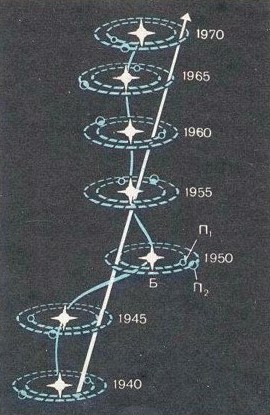
\includegraphics[width=0.4\textwidth]{image.jpg} % Замените 'image.png' на имя вашего файла
\end{figure}

\end{document}
